\begin{figure}
    \centering
    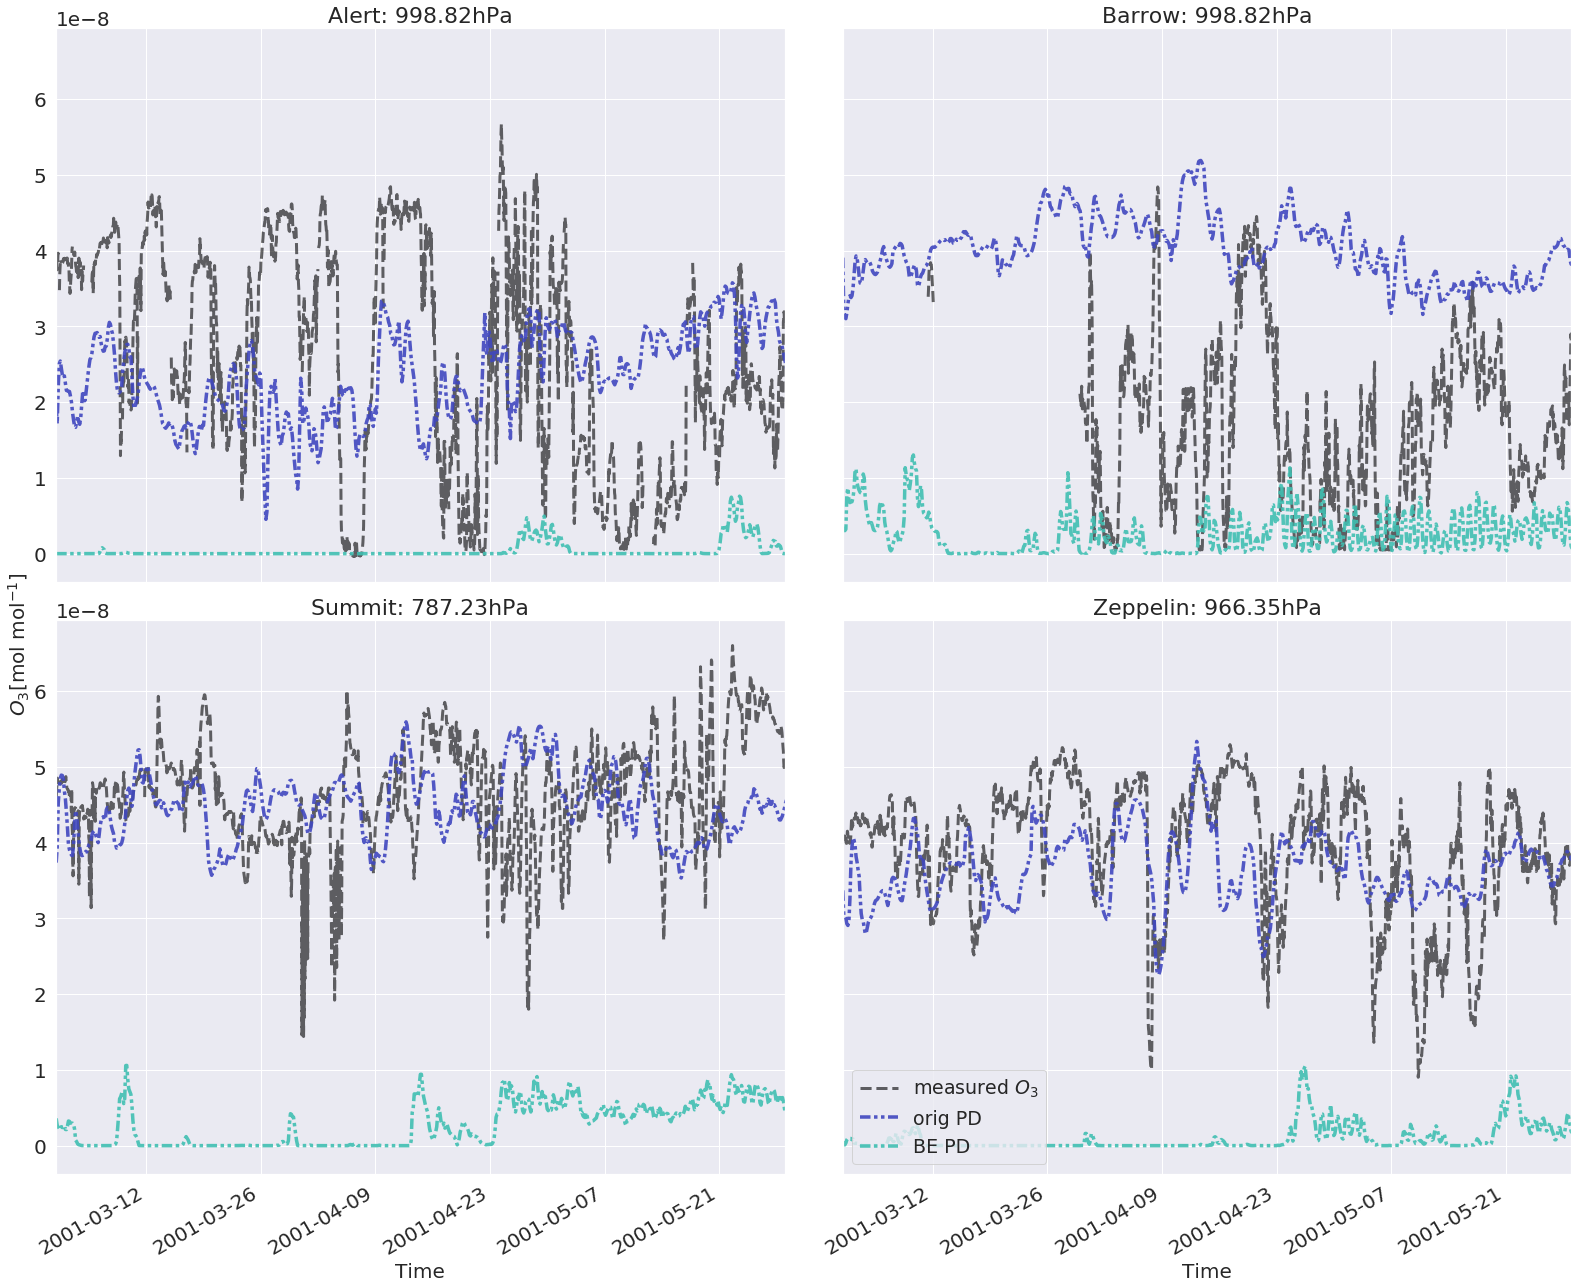
\includegraphics[width = \linewidth]{Chapter6_Results/images/ozone_stationComp_2001/ozone_2001_compObsOrigBE.png}
    \caption{Ozone measurements (black line) and model results from the original CTM3 (Branch \ref{def:origCTM3_PD}) (blue line) and Branch \ref{def:BE_PD} (turquoise line) at the four different stations, Alert (top left), Barrow (top right), Summit (lower left) and Zeppelin (lower right) with available measurements in 2001. Model results were taken from the approximate altitude of the station in hPa. PD = present day, BE = bromine explosion}
    \label{fig:CompObsOrigBE}
\end{figure}